\documentclass[12pt]{article}

\usepackage{fontawesome}
\usepackage{hyperref}
\usepackage{xurl}
\usepackage{graphicx}
\usepackage{float}
\usepackage{fancyvrb}
\usepackage[tagged, highstructure]{accessibility}
\usepackage{bookmark}
\usepackage{enumitem}

\hypersetup{
    colorlinks=false,
    pdfborder={0 0 0},
    pdftitle={Detecting and Managing Infections},
    pdfauthor={Adrianna Holden-Gouveia},
    pdfsubject={Information Security - Lab Assignment},
    pdflang={en-US},
    pdfkeywords={malware cleanup, EICAR test file, antivirus, Task Manager, cleanup kit}
}

% Configure PDF bookmarks for navigation
\bookmarksetup{
    numbered,
    open,
}

% Configure list spacing for better accessibility
\setlist{nosep}



\title{Detecting and Managing Infections}
\author{
        Adrianna Holden-Gouveia \\
        Website: \href{https://aholdengouveia.name}{aholdengouveia.name}\\ 
        \date{\vspace{-5ex}}
        %Email: \href{mailto:admin@aholdengouveia.name}{admin@aholdengouveia.name} \\
%        \faLinkedin{: aholdengouveia} \\
        \faGithub {: aholdengouveia} \\
        \faTwitter {: aholdengouveia} \\
        }

%S\date{\today}


\begin{document}

\maketitle

\section*{Accessibility Notice}
This document is also available in HTML format at:

Link: \href{https://aholdengouveia.name/InfoSec/labs/infections.html}{\textbf{\nolinkurl{https://aholdengouveia.name/InfoSec/labs/infections.html}}}

The HTML version provides enhanced accessibility features including keyboard navigation, screen reader support, responsive design, dark mode support, and high contrast options.

\section*{Learning Outcomes}
By the end of this lab, you will be able to:
\begin{itemize}
    \item Test that antivirus software catches a known threat, using a safe test file
    \item Identify signs of infection on your own computer
    \item Build a cleanup kit with current, trusted tools
    \item Write cleanup steps a home user can follow
\end{itemize}

\section*{Lab Instructions}
Everyone eventually gets asked, ``can you look at my computer? I think it has a virus.'' In this lab, you'll test your antivirus safely, check your own computer for signs of trouble, build a cleanup kit, and write a guide you could actually give to a friend or family member.

\subsection*{Screenshots}
This lab asks for about 8 screenshots. Each screenshot should have your name, term, and year.  One of the easiest ways to do that is make a text document with your name and term/year on your computer and save it to use all term. Any screenshots that don't include this information won't be counted.

\begin{figure}[H]
    \centerline{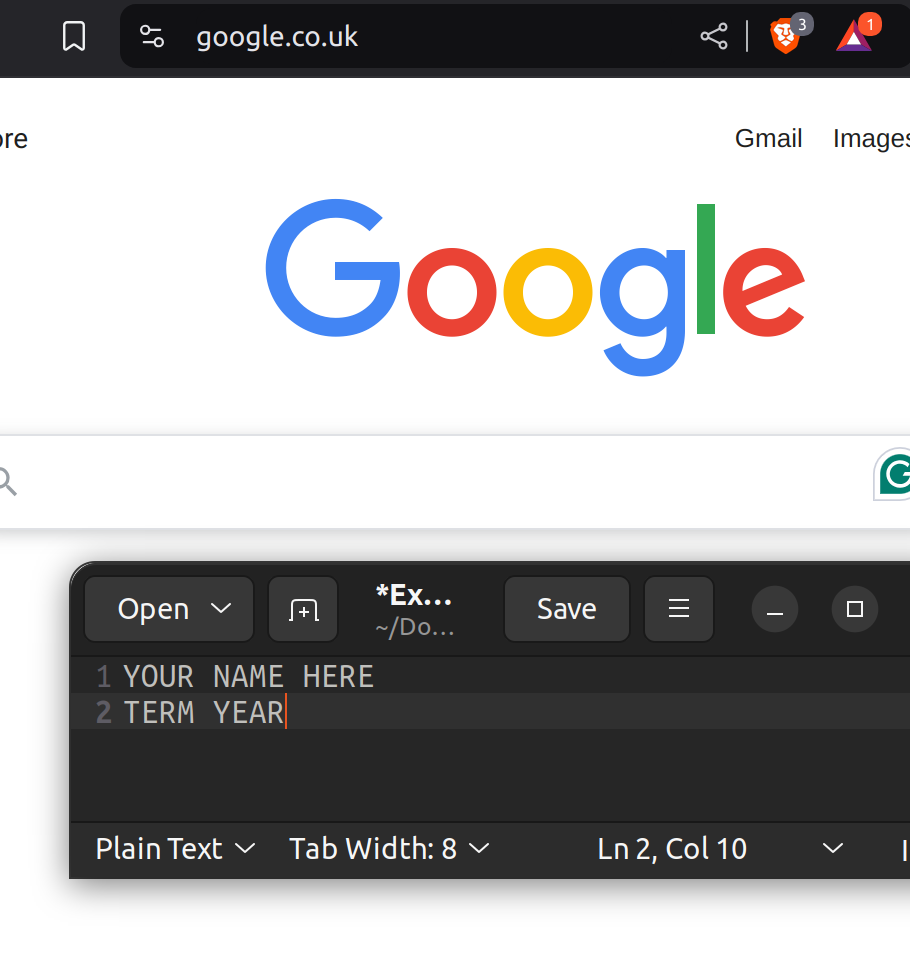
\includegraphics[scale=.2]{ExampleScreenshot.png}}
    \caption{This is an image of what each of your screenshots should look like}
    \alt{Example screenshot: a web browser showing the Google home page, with a small text editor window in front of it that says YOUR NAME HERE and TERM YEAR}
\end{figure}

\textbf{Blur or cover anything sensitive before you turn in a screenshot}, as long as your name and term note still shows, such as your username, email address, or file names that are private.

\subsection*{Part 1: Test Your Antivirus Safely}
The EICAR test file is a harmless file that antivirus programs are built to detect. It isn't a virus, and it doesn't contain any malware. Security teams use it to check that antivirus is working, without using real malware. \textbf{Don't turn off your antivirus to get the file}. Seeing it get blocked is the point.
\begin{enumerate}
    \item Go to the EICAR download page, linked under Resources, and download \texttt{eicar.com.txt}. Take a screenshot of what your computer does, such as a warning, a blocked download, or nothing at all.
    \item Find where your antivirus keeps a record of what it caught, and take a screenshot. On Windows, open Windows Security, then Virus \& threat protection, then Protection history.
    \item If nothing happened, that's a result too. Macs and Chromebooks often don't react to the test file. Test it in your Linux virtual machine instead: download \texttt{eicar.com.txt} in the virtual machine's browser, then run these commands. Installing ClamAV can take a few minutes to download its list of known malware. If \texttt{clamscan} says it can't find the database, wait a few minutes, and try again.
\begin{Verbatim}
sudo apt install clamav
cd Downloads
clamscan eicar.com.txt
\end{Verbatim}
    Take a screenshot of the result. If your computer did catch it, you can skip this question.
    \item Why do security teams use a test file instead of real malware? What did your test tell you about your computer's protection?
\end{enumerate}
Delete the test file when you're done.

\subsection*{Part 2: Check for Signs of Infection}
Look for the signs from the topic page, such as a slow computer, high CPU use, programs you don't recognize, and browser extensions you didn't add.
\begin{itemize}
    \item \textbf{Windows:} press Ctrl, Shift, and Esc to open Task Manager. On the Processes page, sort by CPU. Then open the Startup apps page.
    \item \textbf{Mac:} open Activity Monitor, and sort by CPU. Then open System Settings, General, then Login Items \& Extensions.
    \item \textbf{Chromebook:} press Search and Esc to open Task Manager, and sort by CPU.
    \item \textbf{Browser extensions:} in Chrome, go to \texttt{chrome://extensions}. In Edge, \texttt{edge://extensions}. In Firefox, \texttt{about:addons}. In Safari, open Settings, then Extensions.
\end{itemize}
\begin{enumerate}[start=5]
    \item Take a screenshot of your processes sorted by CPU. What are the top 3, and what does each one do?
    \item Take a screenshot of your startup apps or login items. Do you need all of them to start when your computer starts?
    \item Take a screenshot of your browser extensions. Do you recognize and use all of them?
    \item Pick 2 items from your screenshots that you didn't recognize. Look each one up, and say whether it's safe. Give your source, such as the maker's website or Microsoft's or Apple's support pages. Be careful: some websites that explain process names try to sell you cleanup software.
    \item Based on what you found, does your computer show any signs of infection? Explain.
\end{enumerate}

\subsection*{Part 3: Build a Cleanup Kit}
Make a folder called Cleanup Kit, on a USB drive if you have one, or on your computer if not. Download at least 2 tools into it, only from the official websites linked under Resources:
\begin{itemize}
    \item \textbf{Windows:} Microsoft Safety Scanner, Emsisoft Emergency Kit, or Malwarebytes AdwCleaner. Windows also has a built-in deep scan, the Microsoft Defender Offline scan, which you don't need to download.
    \item \textbf{Mac:} Malwarebytes for Mac, and one Windows tool, so your kit can help someone else.
    \item \textbf{Chromebook:} build a kit for a Windows computer, using 2 of the Windows tools.
\end{itemize}
\begin{enumerate}[start=10]
    \item Take a screenshot of your Cleanup Kit folder.
    \item For one Windows tool, check its digital signature, like you did in the Physical and Device Security lab: right-click it, select Properties, then Digital Signatures. Take a screenshot. If you're on a Mac or Chromebook, explain who the signature should be from, and why it matters.
    \item Microsoft Safety Scanner stops working 10 days after you download it. Why do tools like this need a fresh download each time?
    \item Why should you only download cleanup tools from official websites? Think about the fake AI model on Hugging Face from the topic page.
\end{enumerate}

\subsection*{Part 4: Your Home Cleanup Guide}
\begin{enumerate}[start=14]
    \item Write a one-page guide that a friend or family member could follow if they think their home computer is infected. Write it for someone who isn't good with computers, with numbered steps in your own words. Include:
    \begin{itemize}
        \item The signs that something is wrong
        \item Backing up important files first
        \item Disconnecting from the internet
        \item Running the tools from your Cleanup Kit, with where to download each one
        \item Running a deeper scan, such as the Microsoft Defender Offline scan
        \item Changing passwords afterwards, from a different, clean device
        \item When to stop and get help from a professional, or reinstall the computer
    \end{itemize}
\end{enumerate}
Make it something you'd actually give someone. You're welcome to share it.

\section*{Deliverables}
One file that includes:
\begin{itemize}
    \item Part 1: your screenshots, and your answers
    \item Part 2: your 3 screenshots, and your answers
    \item Part 3: your 2 screenshots, and your answers
    \item Part 4: your home cleanup guide
\end{itemize}

\section*{Resources}
References, a video, a PowerPoint and some notes are available at my website
Link: \href{https://www.aholdengouveia.name/InfoSec/ManagingInfections.html}{\textbf{\nolinkurl{https://www.aholdengouveia.name/InfoSec/ManagingInfections.html}}}

EICAR: the anti-malware test file, for Part 1
Link: \href{https://www.eicar.org/download-anti-malware-testfile/}{\textbf{\nolinkurl{https://www.eicar.org/download-anti-malware-testfile/}}}

Microsoft Safety Scanner, for Part 3
Link: \href{https://learn.microsoft.com/en-us/defender-endpoint/safety-scanner-download}{\textbf{\nolinkurl{https://learn.microsoft.com/en-us/defender-endpoint/safety-scanner-download}}}

Emsisoft Emergency Kit, a free portable scanner, for Part 3
Link: \href{https://www.emsisoft.com/en/emergency-kit/}{\textbf{\nolinkurl{https://www.emsisoft.com/en/emergency-kit/}}}

Malwarebytes AdwCleaner, for adware, for Part 3
Link: \href{https://www.malwarebytes.com/adwcleaner}{\textbf{\nolinkurl{https://www.malwarebytes.com/adwcleaner}}}

Malwarebytes, including Malwarebytes for Mac, for Part 3
Link: \href{https://www.malwarebytes.com/}{\textbf{\nolinkurl{https://www.malwarebytes.com/}}}

Microsoft: Virus and threat protection in the Windows Security app, including the Microsoft Defender Offline scan
Link: \href{https://support.microsoft.com/en-us/windows/security/threat-malware-protection/virus-and-threat-protection-in-the-windows-security-app}{\textbf{\nolinkurl{https://support.microsoft.com/en-us/windows/security/threat-malware-protection/virus-and-threat-protection-in-the-windows-security-app}}}

FTC: Malware: how to protect against, detect, and remove it
Link: \href{https://consumer.ftc.gov/articles/malware-how-protect-against-detect-and-remove-it}{\textbf{\nolinkurl{https://consumer.ftc.gov/articles/malware-how-protect-against-detect-and-remove-it}}}

\end{document}
